\documentclass[a4paper]{article}

\usepackage[utf8]{inputenc}
\usepackage[ngerman]{babel}
\usepackage{graphicx}
\usepackage{pdfpages}

\begin{document}
  \title{VU Objektorientierte Analyse und Design}
  \author{Gruppe 46}
  \date{9.11.2018}
  \maketitle

\section{A1}
\subsection{Klassendiagramm Hausverwaltung}

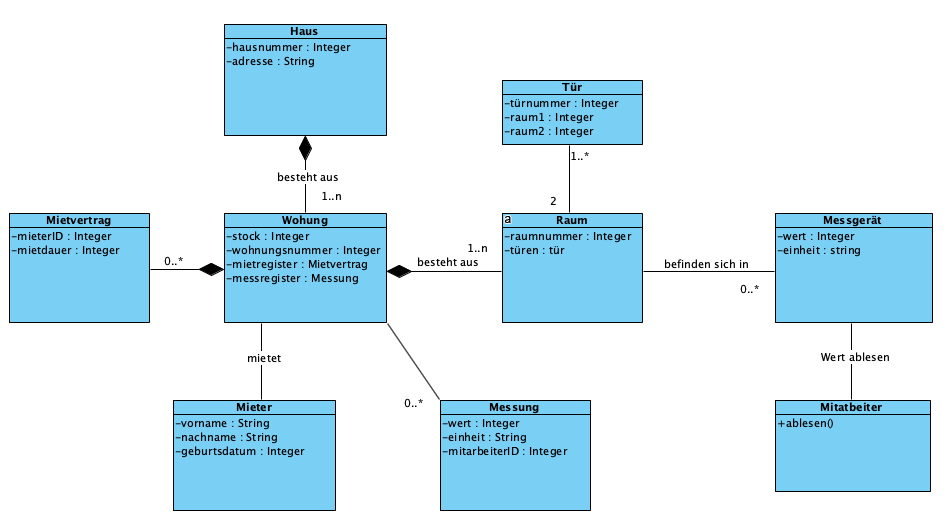
\includegraphics[width=\textwidth]{/home/zdenek/Documents/studium/sem3/OO_Analyse_Design/Project/OAD-2018-2019/Ass2/A1/Aufgabe1.png}


\section{A2}

\subsection{Business Case}

\subsubsection{Problemdefinition}

Die Anwendung T-REC soll es Usern ermöglichen, mit geringem Aufwand ein
den eigenen Interessen und Vorlieben entsprechendes Hotel zu finden. Beim
Planen seines nächsten Urlaubs ist das Angebot naturgemäß sehr groß und es
bedarf eines gewissen Aufwands, um interessante Optionen herauszufiltern. Un-
sere Produkt nimmt dem Anwender diese Arbeit ab und trifft seinen Vorlieben
entsprechend eine Vorauswahl. T-REC bringt also unsere Kunden (Hotels) ihren
Kunden (Urlaubsgäste) ein ordentliches Stück näher.

\subsubsection{Teambeschreibung und Rollen}

\begin{itemize}
\item Stefan Bortolas: Projektmanager
\item Christof Gartner: Analyst
\item Manuel Gußmagg: Usability Tester
\item Christoph Proß: Entwickler
\item Tanja Tatschl: Support
\item Zdenek Zeman: Tester
\end{itemize}

\subsubsection{Meilensteine}

\begin{itemize}
\item Organisation
\item Requirements
\item Projektstrukturplan
\item Aufgabe 1
\item GUI Prototype
\item Use Cases Diagramm
\end{itemize}

\subsubsection{Projektstrukturplan}

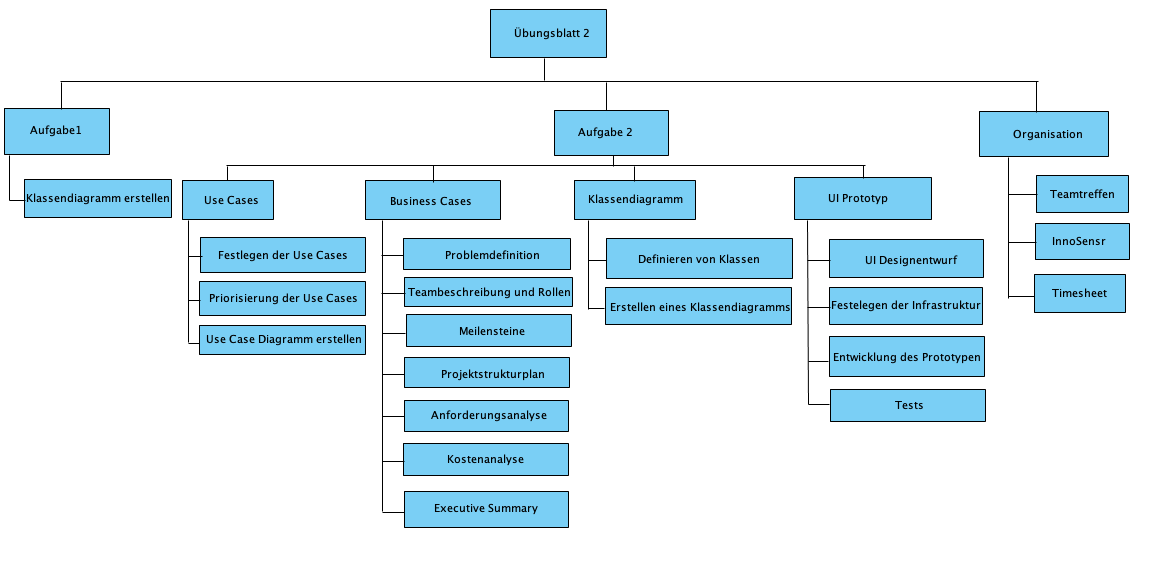
\includegraphics[width=\textwidth]{/home/zdenek/Documents/studium/sem3/OO_Analyse_Design/Project/OAD-2018-2019/Ass2/A2/Projektstrukturplan.png}

\subsubsection{Anforderungsanalyse}

Anforderungen nach Relevanz gelistet:

\begin{itemize}
\item Hotel bewerten
\item Objekte suchen
\item Aktivitäten festlegen
\item Anmelden
\item Datenbank auswerten
\item Registrieren
\item Interessensprofil verwalten
\item Statistiken anzeigen
\item Accounts verwalten
\item Empfehlungen erhalten
\item Hoteldaten verwalten
\end{itemize}

\subsubsection{Executive Summary}

Dieses Dokument wurde erstellt, um unserem Kunden die strukturierte Vorge-
hensweise in der Inseption-Phase des Projekts zu erläutern.

\subsection{Use Cases}



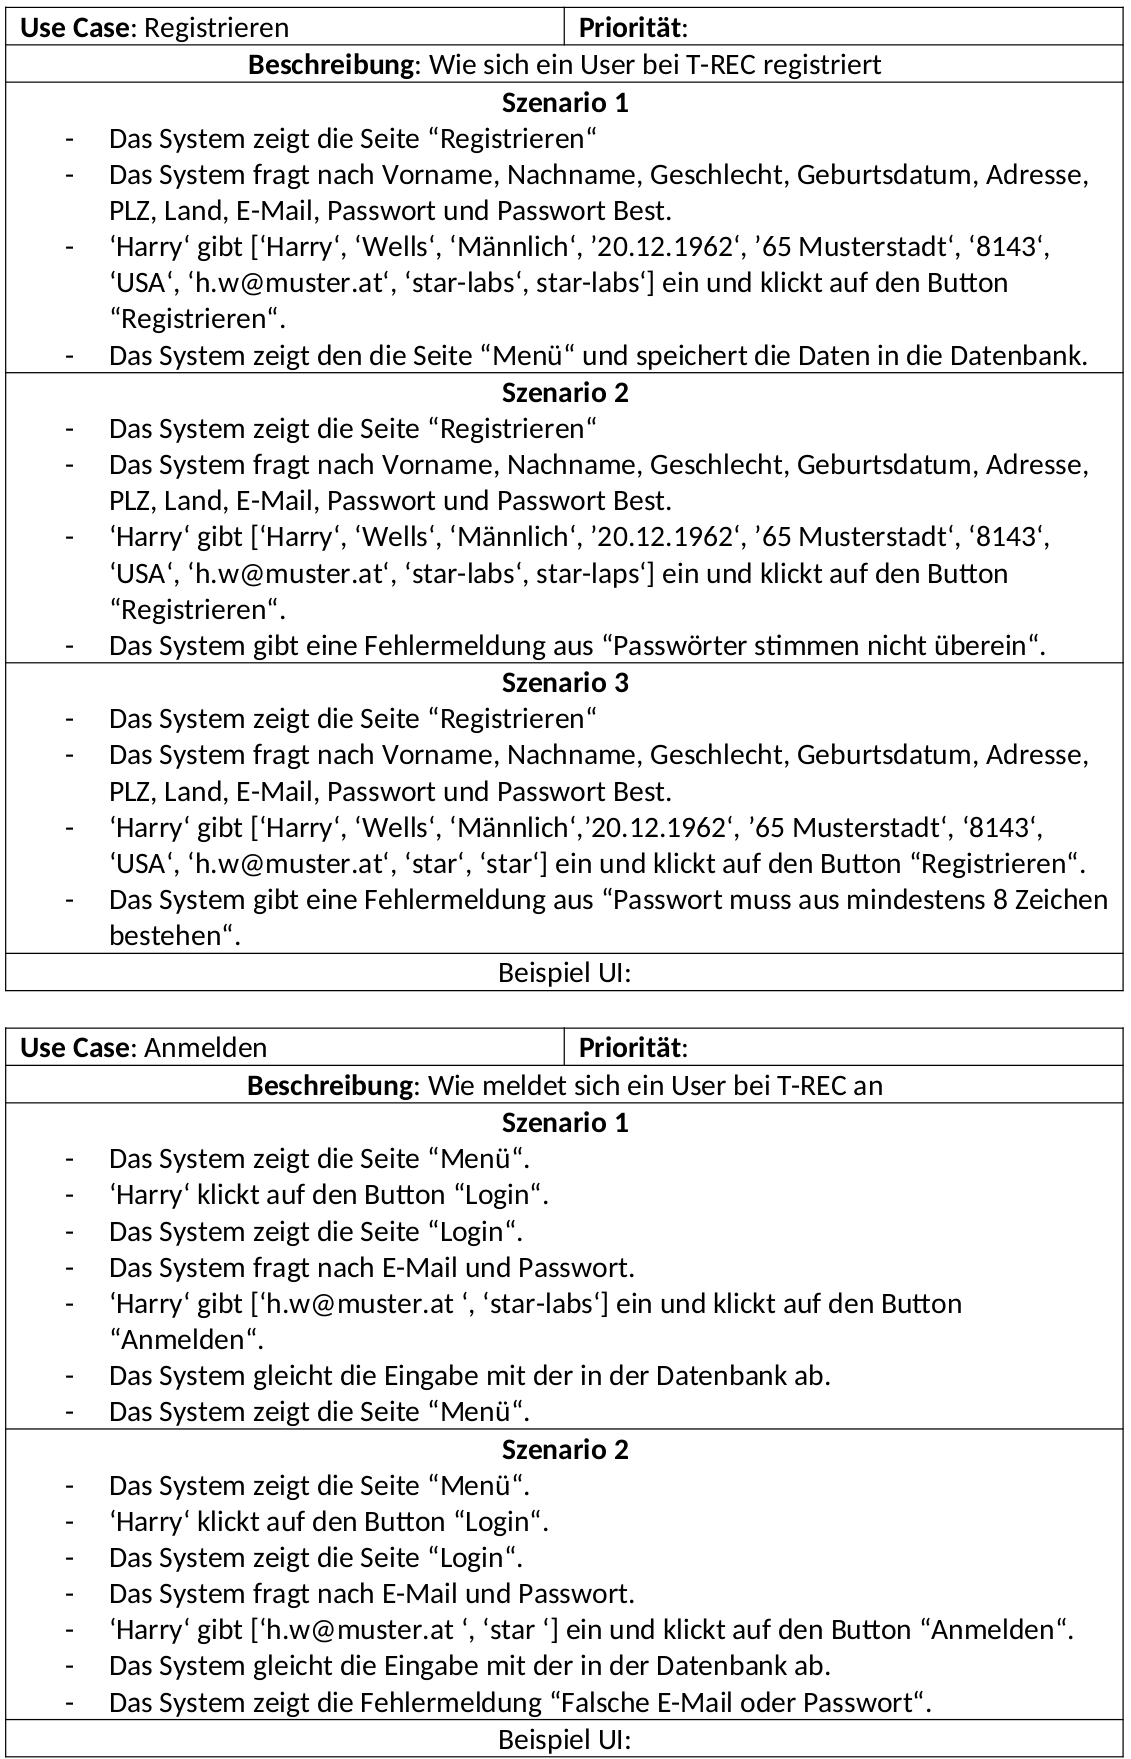
\includegraphics[width=\textwidth]{/home/zdenek/Documents/studium/sem3/OO_Analyse_Design/Project/OAD-2018-2019/Ass2/temp/use_cases_descr0.jpg}
\newpage
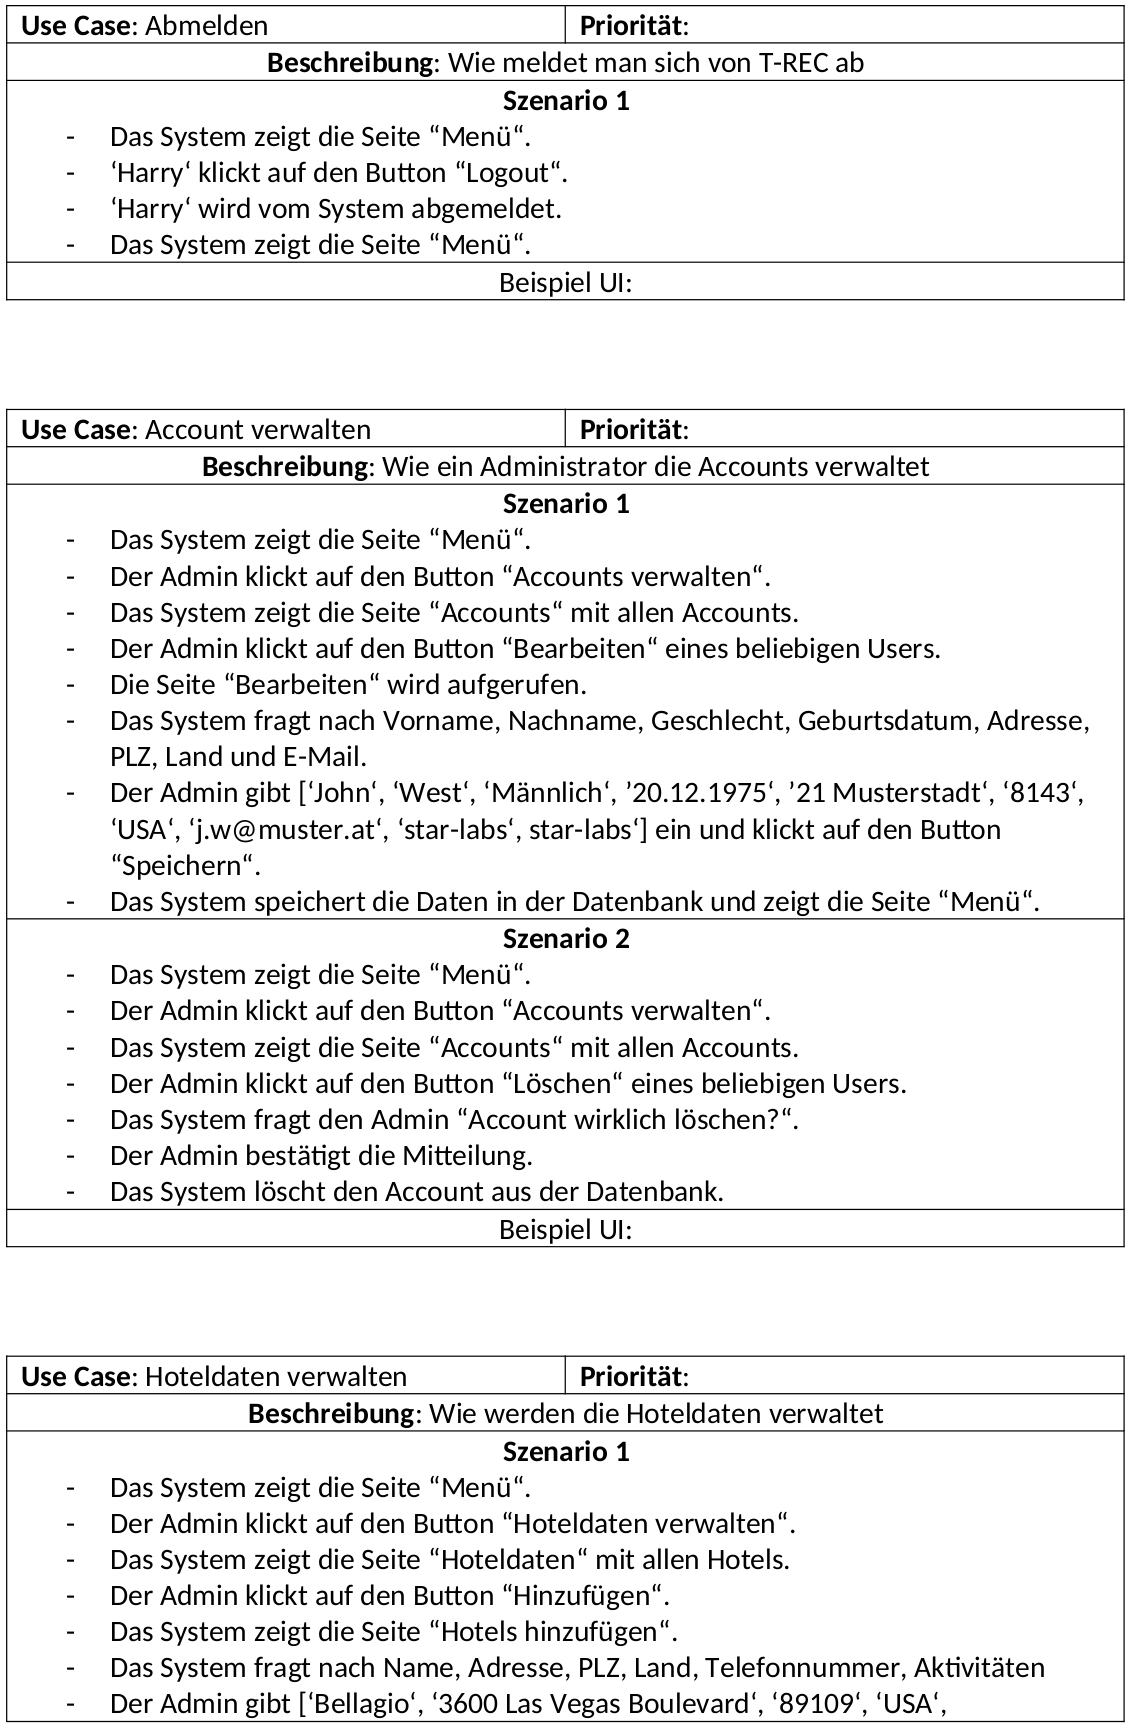
\includegraphics[width=\textwidth]{/home/zdenek/Documents/studium/sem3/OO_Analyse_Design/Project/OAD-2018-2019/Ass2/temp/use_cases_descr1.jpg}
\newpage
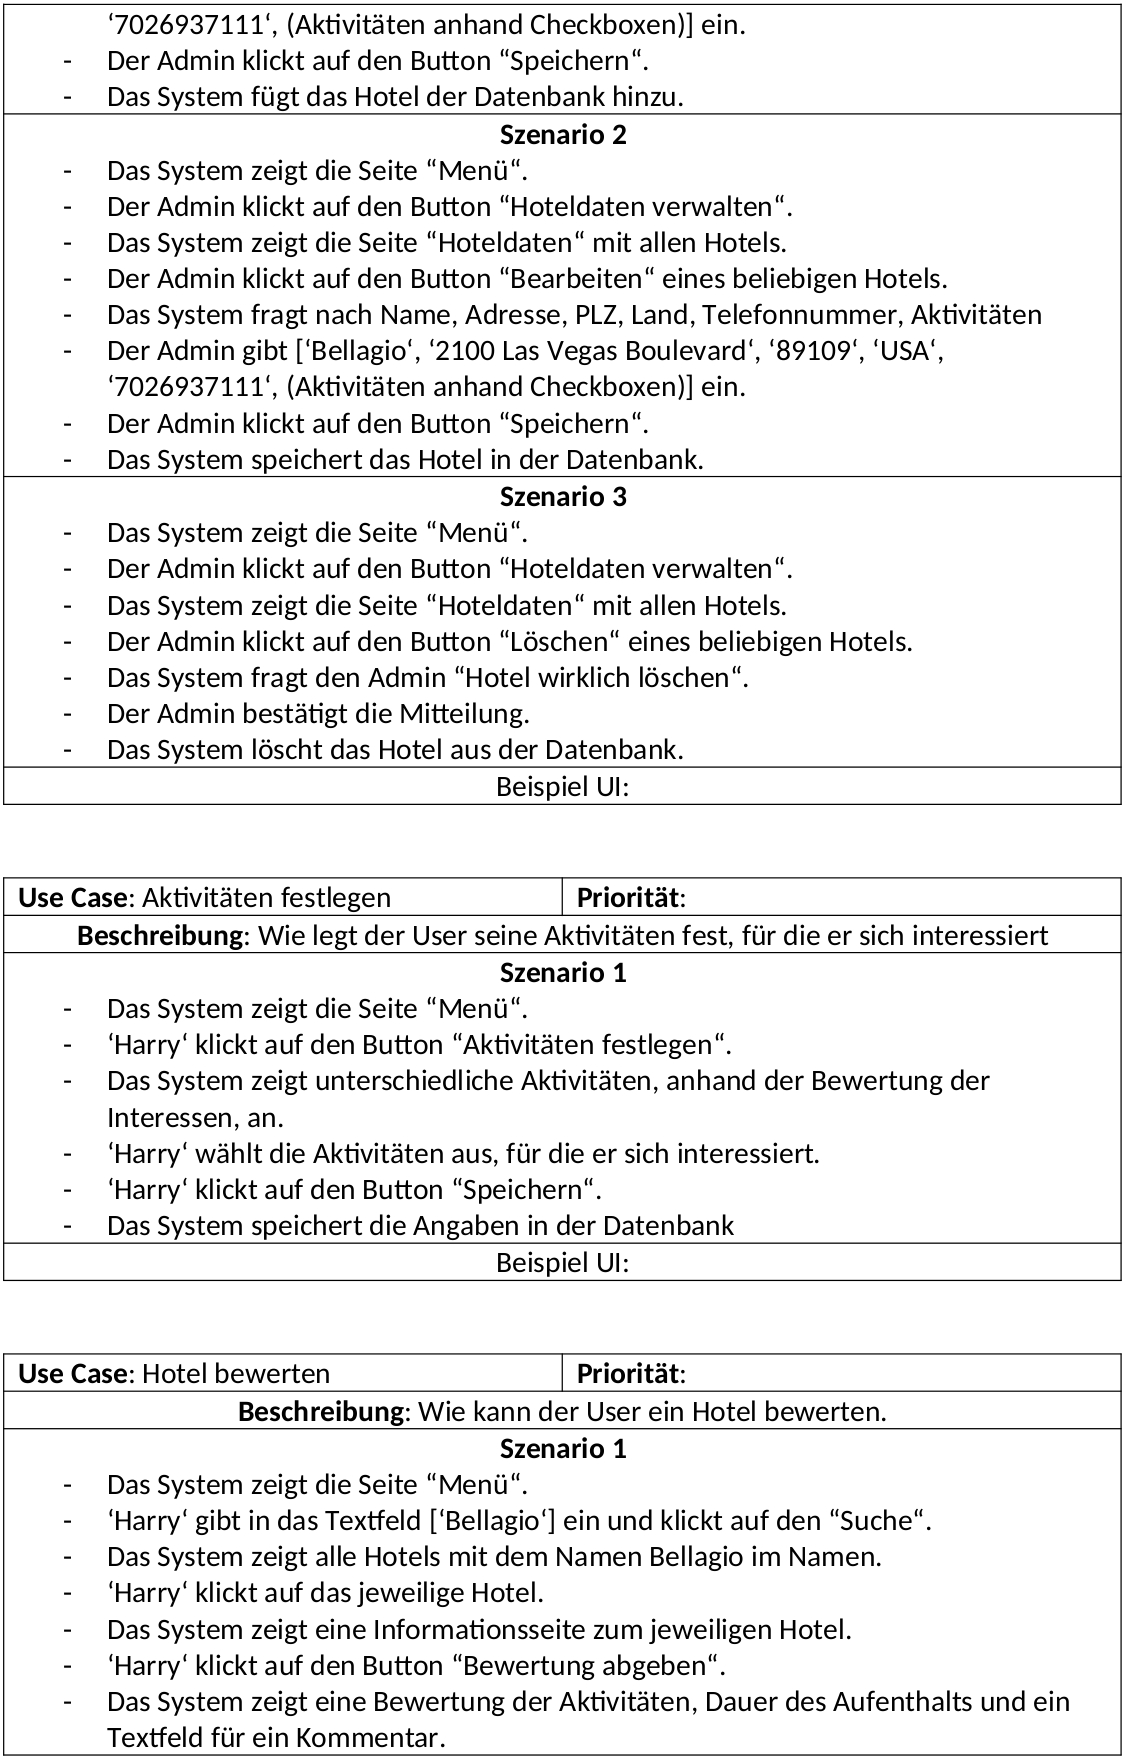
\includegraphics[width=\textwidth]{/home/zdenek/Documents/studium/sem3/OO_Analyse_Design/Project/OAD-2018-2019/Ass2/temp/use_cases_descr2.jpg}
\newpage
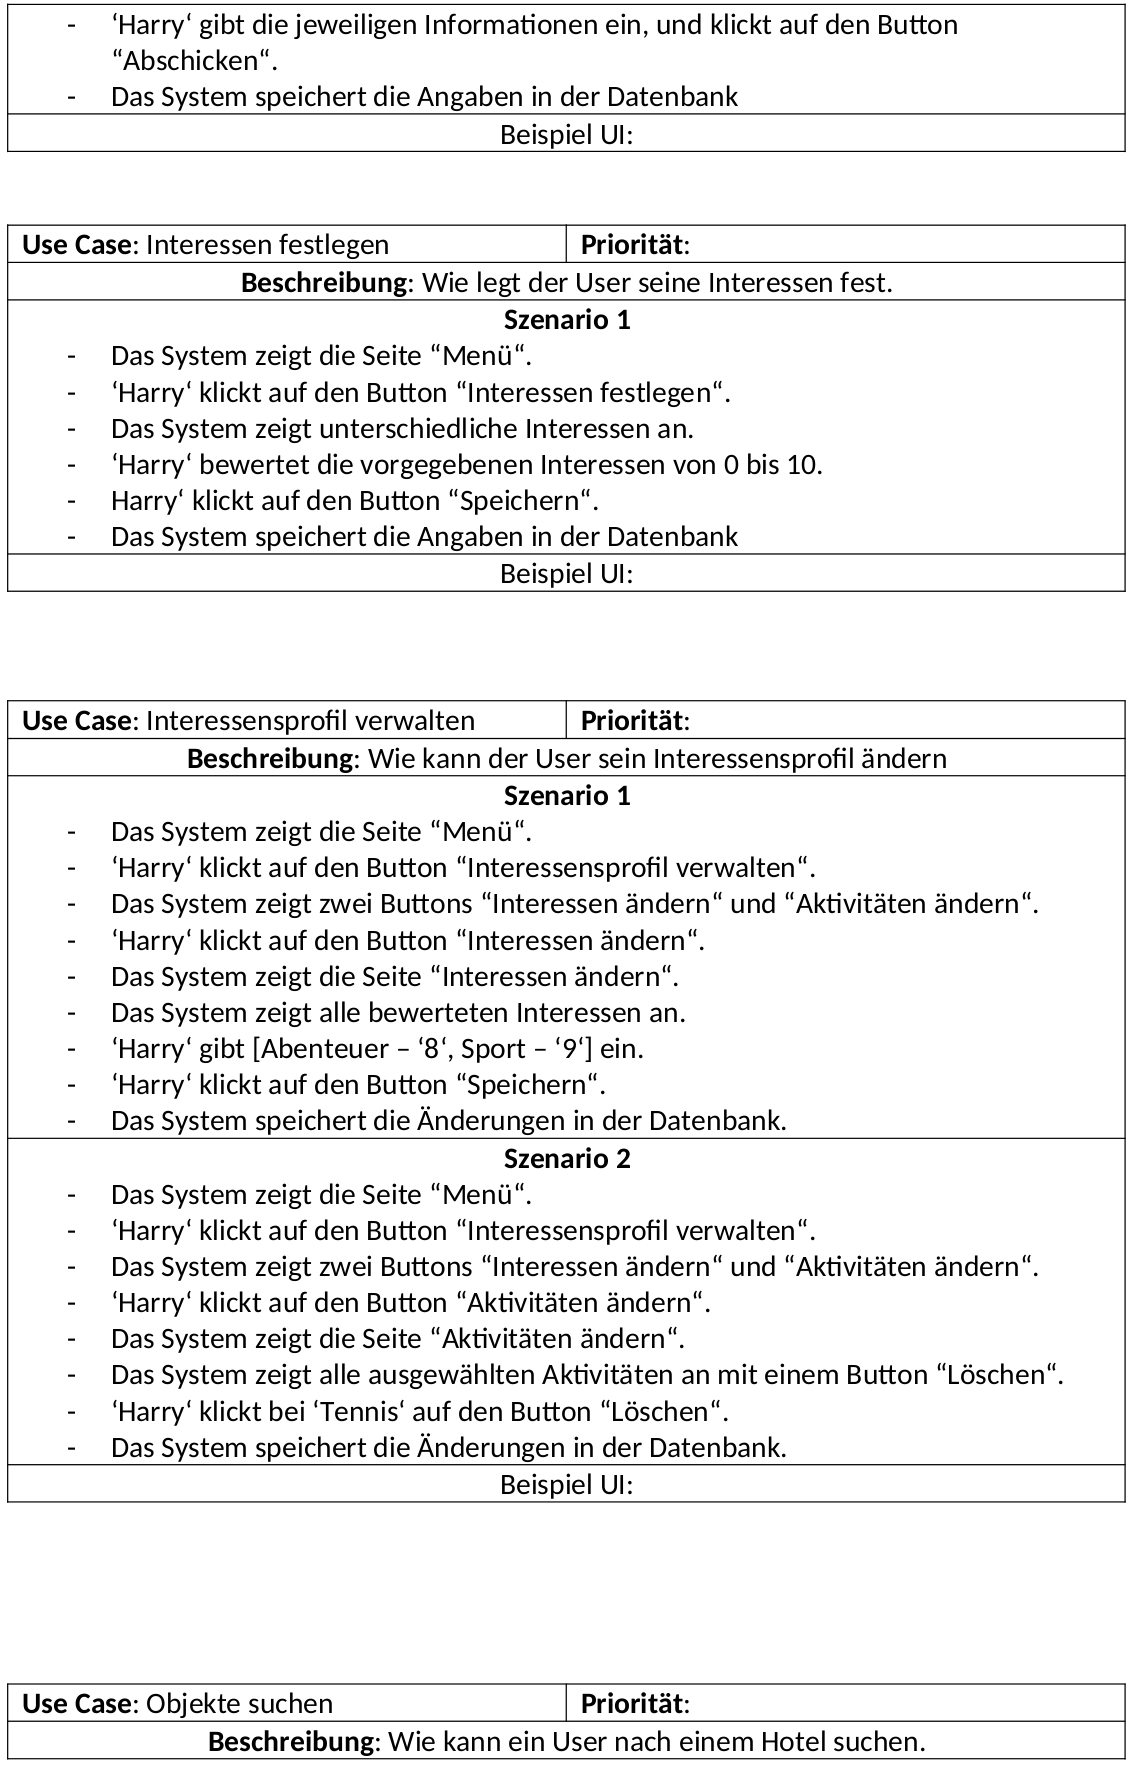
\includegraphics[width=\textwidth]{/home/zdenek/Documents/studium/sem3/OO_Analyse_Design/Project/OAD-2018-2019/Ass2/temp/use_cases_descr3.jpg}
\newpage
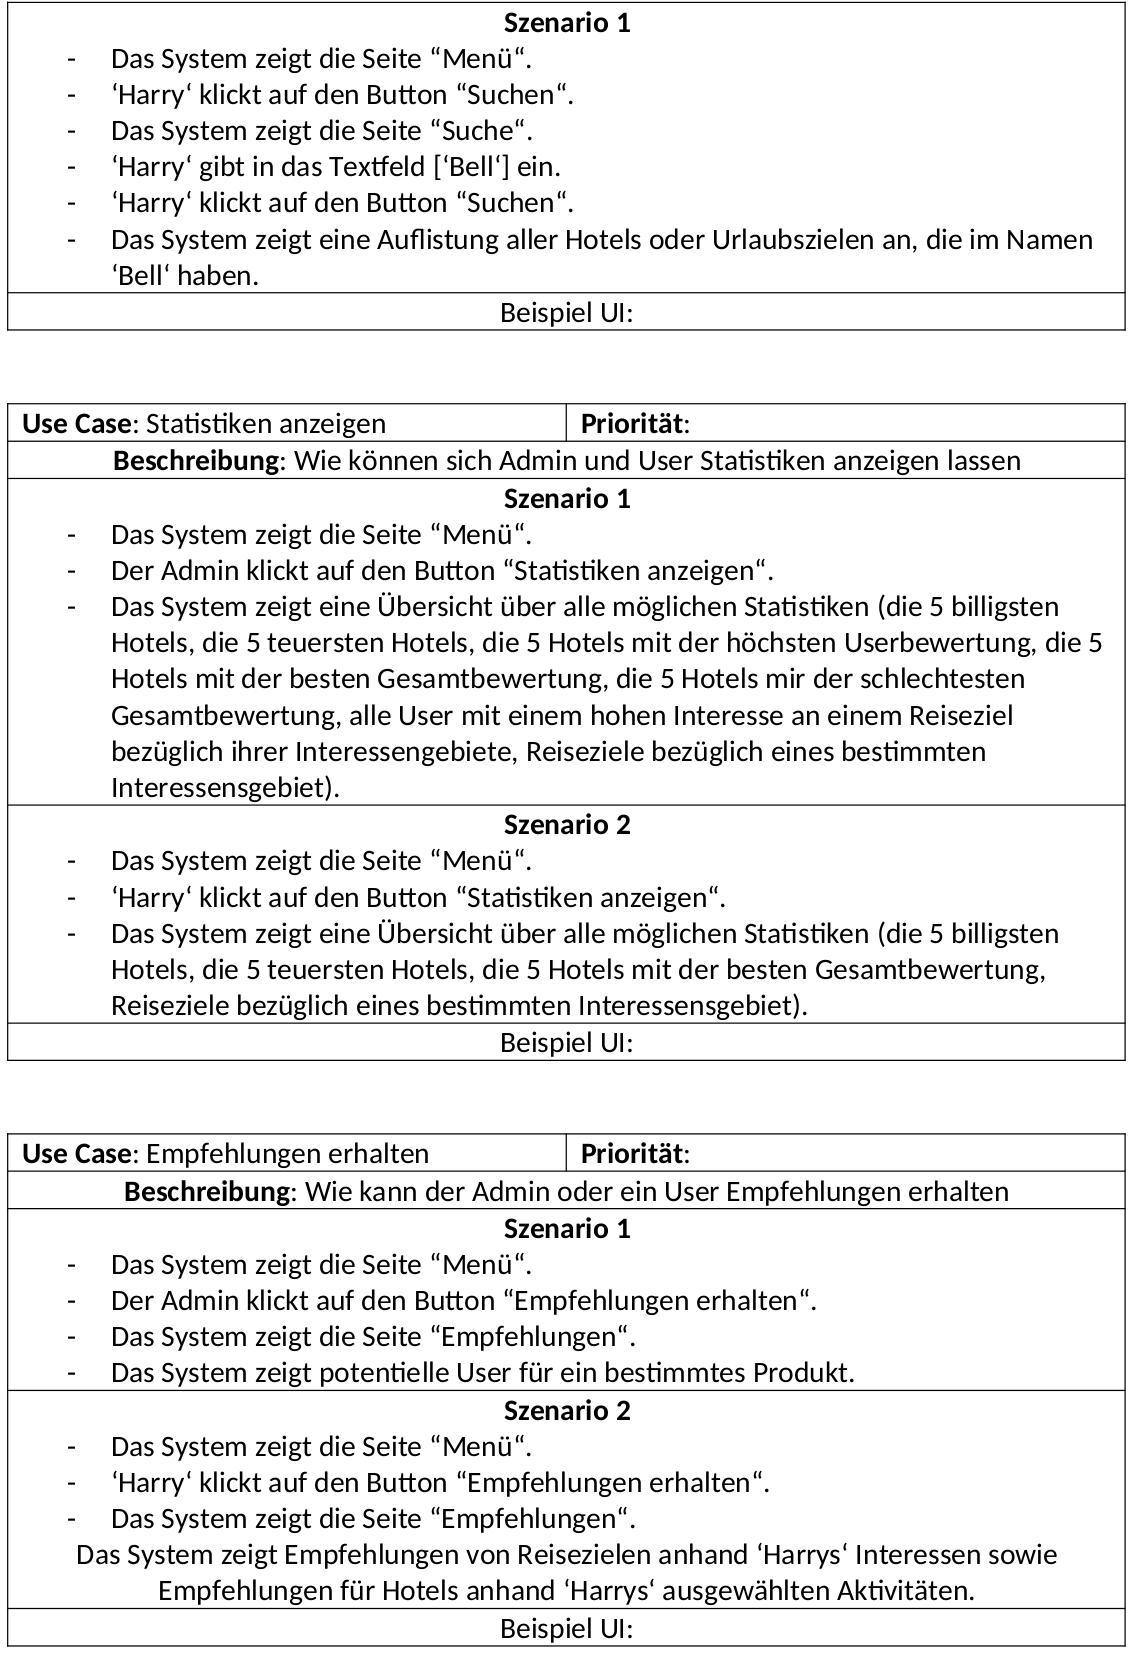
\includegraphics[width=\textwidth]{/home/zdenek/Documents/studium/sem3/OO_Analyse_Design/Project/OAD-2018-2019/Ass2/temp/use_cases_descr4.jpg}
\newpage
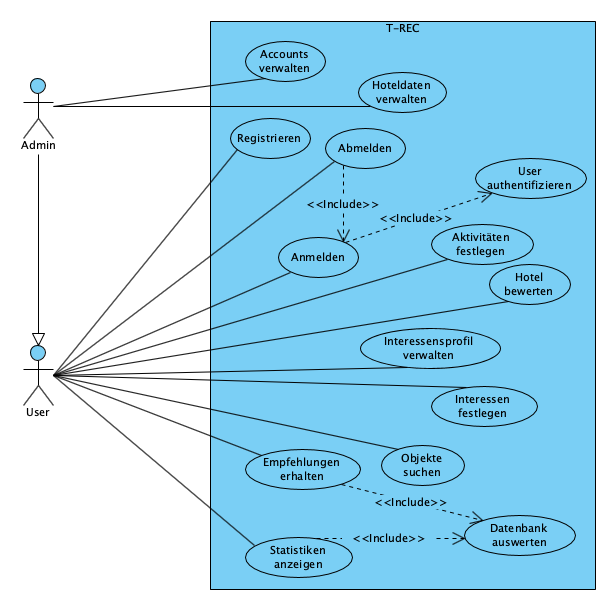
\includegraphics[width=\textwidth]{/home/zdenek/Documents/studium/sem3/OO_Analyse_Design/Project/OAD-2018-2019/Ass2/A2/Use-Case-Bild.png}

\newpage

\subsection{GUI}

Screenshots des ersten Prototypen des Graphical User Interface

\begin{figure}[h]
\centering
\caption{Home}
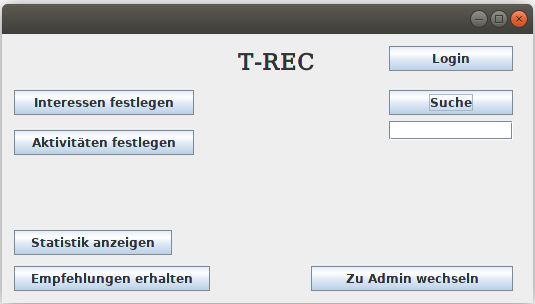
\includegraphics[width=0.5\textwidth]{/home/zdenek/Documents/studium/sem3/OO_Analyse_Design/Project/OAD-2018-2019/Ass2/A2/Ui-Screenshots/Selection_017.png}
\end{figure}

Von hier aus gelangt man zu den meisten Funktionen von T-REC.
Da das Einloggen noch nicht implementiert wurde, gelangt man zur Administrator-Ansicht über einen Knopf.


\begin{figure}[h]
\centering
\caption{Anmeldung}
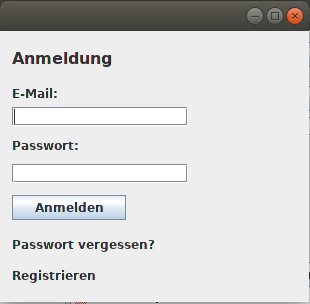
\includegraphics[width=0.5\textwidth]{/home/zdenek/Documents/studium/sem3/OO_Analyse_Design/Project/OAD-2018-2019/Ass2/A2/Ui-Screenshots/Selection_007.png}
\end{figure}

Bei der Anmeldung gibt man seine E-Mail und sein Passwort ein, das man bei der Registrierung angegeben hat. Weiters ist es möglich sein Passwort per Mail geschickt zu bekommen sowie sich überhaupt mal zu registrieren.

\begin{figure}[h]
\centering
\caption{Registrierung}
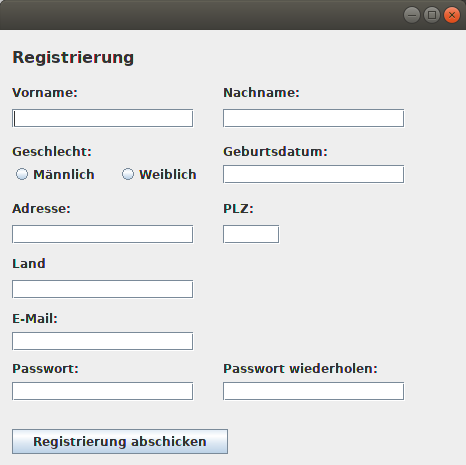
\includegraphics[width=0.5\textwidth]{/home/zdenek/Documents/studium/sem3/OO_Analyse_Design/Project/OAD-2018-2019/Ass2/A2/Ui-Screenshots/Selection_008.png}
\end{figure}

Bei der Registrierung muss der Kunde neben den Zugangsdaten verschiedene persönliche Daten angeben, die es später den Hotelbesitzern erleichtern gezielt Kunden zu finden die sie bewerben können.


\begin{figure}[h]
\centering
\caption{Suche}
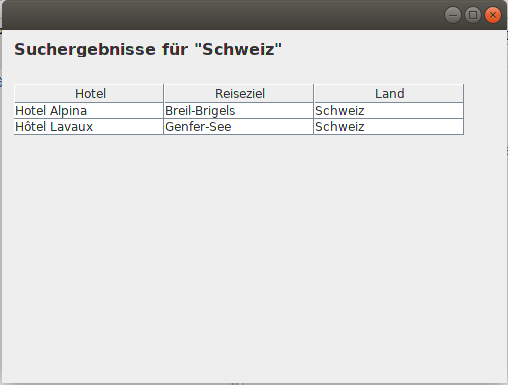
\includegraphics[width=0.5\textwidth]{/home/zdenek/Documents/studium/sem3/OO_Analyse_Design/Project/OAD-2018-2019/Ass2/A2/Ui-Screenshots/Selection_009.png}
\end{figure}

Mit der Suchfunktion können Länder, Reiseziele und Hotels aus der Datenbank gefiltert werden. Klickt man auf ein Ergebnis, werden Informationen zum jeweiligen Hotel angezeigt.


\begin{figure}[h]
\centering
\caption{Empfehlungen}
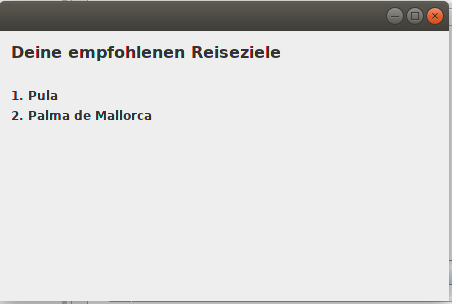
\includegraphics[width=0.5\textwidth]{/home/zdenek/Documents/studium/sem3/OO_Analyse_Design/Project/OAD-2018-2019/Ass2/A2/Ui-Screenshots/Selection_010.png}
\end{figure}

In diesem Fenster werden dem Kunden jene Reiseziele vorgeschlagen, die am Besten zu seinen Präferenzen passen. Beim Klick auf ein Reiseziel werden dann die Hotels angezeigt die wiederum am Besten zum Kunden passen.

\begin{figure}[h]
\centering
\caption{Statistiken}
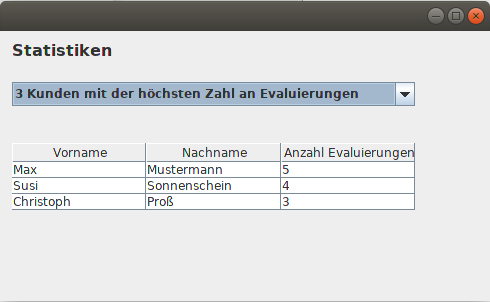
\includegraphics[width=0.5\textwidth]{/home/zdenek/Documents/studium/sem3/OO_Analyse_Design/Project/OAD-2018-2019/Ass2/A2/Ui-Screenshots/Selection_011.png}
\end{figure}

Diese Funktion ermöglicht es die Datenbank nach verschiedenen Kriterien auszuwerten.
Die Ergebnisse werden tabellarisch ausgegeben.

\begin{figure}[h]
\centering
\caption{Aktivitäten}
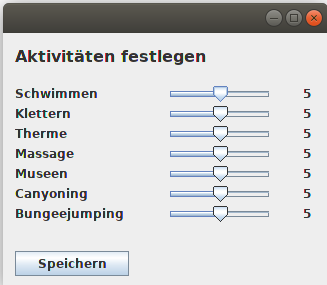
\includegraphics[width=0.5\textwidth]{/home/zdenek/Documents/studium/sem3/OO_Analyse_Design/Project/OAD-2018-2019/Ass2/A2/Ui-Screenshots/Selection_012.png}
\end{figure}

In diesem Fenster kann der Kunde angeben welche konkreten Aktivitäten er wie gerne ausübt. 

\begin{figure}[h]
\centering
\caption{Interessen}
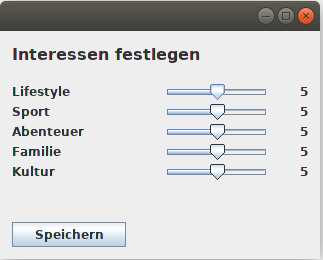
\includegraphics[width=0.5\textwidth]{/home/zdenek/Documents/studium/sem3/OO_Analyse_Design/Project/OAD-2018-2019/Ass2/A2/Ui-Screenshots/Selection_014.png}
\end{figure}

Hierbei kann der Kunde seine persönlichen Vorlieben für bestimmte Themen angeben.

\begin{figure}[h]
\centering
\caption{Hoteldetails}
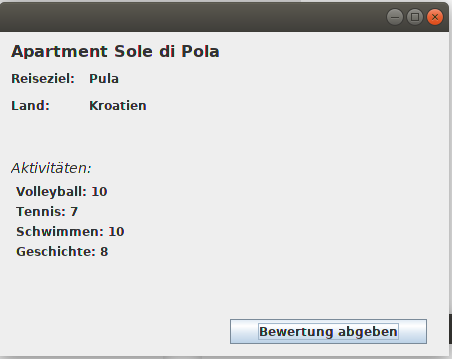
\includegraphics[width=0.5\textwidth]{/home/zdenek/Documents/studium/sem3/OO_Analyse_Design/Project/OAD-2018-2019/Ass2/A2/Ui-Screenshots/Selection_015.png}
\end{figure}

Hier werden die relevanten Informationen (Reiseziel, Land und Aktivitäten) zu einem Hotel angezeigt. Weiters ist es möglich über einen Knopf das Hotel zu bewerten.

\begin{figure}[h]
\centering
\caption{Hotelbewertung}
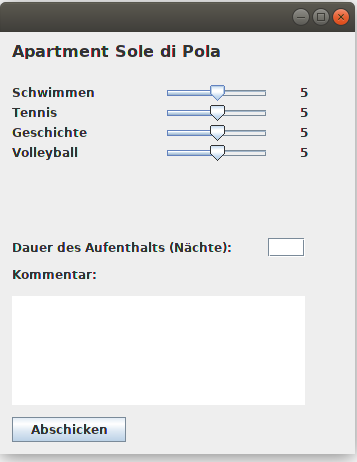
\includegraphics[width=0.5\textwidth]{/home/zdenek/Documents/studium/sem3/OO_Analyse_Design/Project/OAD-2018-2019/Ass2/A2/Ui-Screenshots/Selection_016.png}
\end{figure}

Dabei lassen sich die angebotenen Aktivitäten des Hotels bewerten und man kann die Dauer des Aufenthalts angeben sowie einen Kommentar hinterlassen.


\end{document}
